\documentclass[dtu]{dtuarticle}
\usepackage{parskip} % use enters instead of indents

\newcommand{\todo}[1]{\color{red}[TODO: #1]\color{black}}
\newcommand*\chem[1]{\ensuremath{\mathrm{#1}}}
\usepackage{amsmath}
\usepackage{bm} % bold ITALIC math (for vectors!)
\usepackage{siunitx}
\sisetup{
	per-mode=fraction,
	detect-weight = true,
	detect-family = true,
	separate-uncertainty=true, % Dit is voor de plus-minus
	output-decimal-marker={.}
}

\usepackage{subcaption}

\title{Machine Learning Project 1}
\subtitle{Data: Feature extraction, and visualization}
\author{Group 94}
\course{02452 Machine Learning}
\address{
	DTU Compute \\
	Fall 2025
}
\date{\today}


\begin{document}

	\maketitle

	%	\begin{table}[h!]
		%		\renewcommand{\arraystretch}{1.1} % make the spacing a bit nicer
		%		\centering
		%		\begin{tabular}{l | l}
			%			\textbf{Name}                 & \textbf{Student number} \\ \hline\hline
			%			Vincent Van Schependom        & s251739                 \\ \hline
			%			Diego Armando Mijares Ledezma & s251777                 \\ \hline
			%			Albert Joe Jensen             & s204601
			%		\end{tabular}
		%		\caption{Group members.}
		%		\label{table:members}
		%	\end{table}
	%
	%	\begin{table}[h!]
		%		\renewcommand{\arraystretch}{1.1} % make the spacing a bit nicer
		%		\centering
		%		\begin{tabular}{l | *{3}{|l}}
			%			\textbf{Task} & \textbf{Vincent} & \textbf{Diego} & \textbf{Albert} \\ \hline\hline
			%			Section 1     & 30\%             & 30\%           & 40\%            \\ \hline
			%			Section 2     & 40\%             & 30\%           & 30\%            \\ \hline
			%			Section 3     & 30\%             & 40\%           & 30\%            \\ \hline
			%			Section 4     & 30\%             & 30\%           & 40\%			\\ \hline
			%			\LaTeX        & 90\%             & 5\%           & 5\%
			%		\end{tabular}
		%		\caption{Contributions \& responsabilities table.}
		%		\label{table:contributions}
		%	\end{table}

	\begin{table}[h!]
		\renewcommand{\arraystretch}{1.2}
		\begin{subtable}{.58\textwidth}
			\begin{tabular}{l | l}
				\textbf{Name}                 & \textbf{Student number} \\ \hline\hline
				Vincent Van Schependom        & s251739                 \\ \hline
				Diego Armando Mijares Ledezma & s251777                 \\ \hline
				Albert Joe Jensen             & s204601
			\end{tabular}
			\caption{Group members.}
			\label{table:members}
		\end{subtable}
		\begin{subtable}{.4\textwidth}
			\begin{tabular}{l | *{3}{|r}}
				\textbf{Task} & \textbf{Vincent} & \textbf{Diego} & \textbf{Albert} \\ \hline\hline
				Section 1     & 40\%             & 0\%            & 60\%            \\ \hline
				Section 2     & 30\%             & 50\%           & 20\%            \\ \hline
				Section 3     & 100\%             & 0\%           & 0\%            \\ \hline
				\LaTeX        & 95\%             & 5\%            & 0\%
			\end{tabular}
			\caption{Contributions \& responsabilities table.}
			\label{table:contributions}
		\end{subtable}
		\caption{Group information \& work distribution.}
	\end{table}

	\section*{Introduction}

	The objective of this report is to apply the methods that were discussed during the first
	section of the course \textit{Machine Learning} \cite{book} to a chosen dataset. The aim is to get
	a basic understanding of the data prior to the further analysis (project report 2).

	The particular dataset that is being investigated is the \textit{Glass Identification} dataset from 1987 by B. German \cite{dataset}. Table \ref{table:members} lists our full names and student numbers, while Table \ref{table:contributions} shows an overview of the contribution of each team member.

	\tableofcontents

	\newpage

	\section{The \textit{Glass Identification} dataset}

	The Glass Identification dataset comes from forensic science research in the 1980s, originally compiled at the Institute of Forensic Medicine, with support from the UCI Machine Learning Repository \cite{dataset}. It was created to help develop methods for identifying types of glass found at crime scenes, such as window glass, containers, or headlamps, based on their chemical makeup.

	For each of the 214 observations, the measured attributes are the glass \texttt{type}, the refractive index (\texttt{RI}) and 8 different oxides, all of which can be seen in Table \ref{table:attributes}.

%	The dataset has been widely shared since its inclusion in the UCI Repository in 1987, and it remains a popular benchmark for testing classification methods in research and teaching.

	\subsection{Previous analysis of the data}

	Several studies have analysed the dataset to improve multi-class classification performance. Zhou et al. applied machine learning techniques in 2023, focusing on optimising Support Vector Machines (SVM) through grid search and Bayesian methods \cite{zhou}. Their optimised SVM model achieved a remarkably high accuracy of 99.25\%, outperforming baseline models such as logistic regression, and demonstrated strong predictive ability when only chemical composition was available.

	In contrast, Bhowmick and Saha concentrated on addressing class imbalance and noisy data, also in 2023 \cite{bhowmick}. They removed outliers using interquartile range filtering, applied ReliefF feature ranking, and balanced classes with SMOTE before training an inverse-distance-weighted k-nearest-neighbor (kNN) classifier. Their improved pipeline reached 78.9\% accuracy with an $F$-measure of 0.791, showing how preprocessing can boost kNN’s effectiveness on this imbalanced dataset.

	\subsection{Goals and \textit{main machine learning aim}}

%	\todo{Explain, in the context of your problem of interest, what you hope to accom-
%		plish/learn from the data using these techniques?}
%
%	\todo{Explain which attribute you wish to predict in the regression based on which
%		other attributes?}
%
%	\todo{Which class label will you predict based on which other attributes in the classi-
%		fication task?}

	The objective is to build models for both regression and classification. For the \textit{regression task}, the target variable will be the Refractive Index (\texttt{RI}), predicted using eight oxides that were measured for each observation. For the \textit{classification task}, the target variable is the glass type (\texttt{type}), which is divided into seven distinct classes. This label will be predicted based on the other attributes, namely the refractive index of the glass and its measured oxide composition

	Since the dataset is inherently structured around glass type classification, it is clear that the \textit{main machine learning aim} of this project is classification, while regression serves as a secondary task.

	\section{A close look at the different attributes}

%	``Assignment: \textit{Describe if the attributes are discrete/continuous and whether they are nominal/or-
%		dinal/interval/ratio.}''

	\subsection{Feature Types}

	The glass type is, of course, a categorical, \textit{nominal} variable, since no glass type is considered `better' or `worse' than another.

	The oxide components are measured in terms of weight percentage in the corresponding oxide, and are classified as \textit{continuous}, \textit{ratio} variables: a value of zero (e.g., 0.0\% Ba) signifies a true absence of that component, making multiplicative comparisons (ratios) meaningful. The refractive index (\texttt{RI}), though also continuous, is an \textit{interval} variable. This is because it is calculated as \(\texttt{RI} = \frac{c}{v}\) where \(c\) is the speed of light in vacuum and \(v\) is the speed of light in the medium. The existence of a true zero would imply infinite light speed so \texttt{RI} cannot be considered ratio-scaled.

	It should be noted that the oxide components collectively form \textit{compositional data}, meaning their values are statistically interdependent because they represent parts of a whole (i.e., they sum to approximately 100\% for each glass sample). This inherent interdependence can influence statistical modeling.

	\subsection{Need for scaling}

	\label{section:scaling}

	Despite the compositional nature, we should definitely scale the oxide features, primarily due to the significant disparity in their numerical ranges. This can be seen from the summary statistics in Table \ref{table:summary-stats}, as well as on the unscaled boxplots in Figure \ref{fig:unscaled-boxplots}. For example, \texttt{Si} (Silicon) often has values around 72\%, whereas \texttt{Fe} (Iron) and \texttt{Ba} (Barium) frequently register values close to 0.0\%. If these features were used in their raw form, distance-based machine learning algorithms (such as $k$-Nearest Neighbors or $k$-Means Clustering) would be unfairly dominated by features with the largest magnitudes, such as \texttt{Si} or \texttt{Ca}.

	\begin{table}
		\centering
		%\renewcommand{\arraystretch}{1.3} % make the spacing a bit nicer
		\begin{tabular}{l|l|l}
			\textbf{Attribute} & \textbf{Description}                    & \textbf{Type of variable} \\ \hline \hline
			\texttt{ID}        & Observation ID (excluded from analysis) & Numeric (discrete)        \\ \hline
			\texttt{RI}        & Refractive Index                        & Continuous                \\ \hline
			\texttt{Na}        & Sodium oxide ($\chem{Na_2 O}$)          & Continuous                \\ \hline
			\texttt{Mg}        & Magnesium oxide ($\chem{Mg O}$)         & Continuous                \\ \hline
			\texttt{Al}        & Aluminum oxide ($\chem{Al_2 O_3}$)      & Continuous                \\ \hline
			\texttt{Si}        & Silicon oxide ($\chem{Si O_2}$)         & Continuous                \\ \hline
			\texttt{K}         & Potassium oxide ($\chem{K_2 O}$)        & Continuous                \\ \hline
			\texttt{Ca}        & Calcium oxide ($\chem{Ca O }$)          & Continuous                \\ \hline
			\texttt{Ba}        & Barium oxide ($\chem{Ba O}$)            & Continuous                \\ \hline
			\texttt{Fe}        & Iron oxide ($\chem{Fe_2 O_3}$)          & Continuous                \\ \hline
			\texttt{type}      & Type of glass                           & Nominal                   \\
		\end{tabular}
		\caption{The 10 studied attributes, along with the observation ID, which was excluded from the analysis.}
		\label{table:attributes}
	\end{table}

	\begin{table}
		\centering
		%\renewcommand{\arraystretch}{1.3} % make the spacing a bit nicer
		\begin{tabular}{r|l|l}
			\textbf{} & \textbf{Abbreviation in dataset} & \textbf{Description}                 \\ \hline\hline
			1 & \texttt{BW-FP}                   & Building Window, Float Processed     \\ \hline
			2 & \texttt{BW-NFP}                  & Building Window, Non Float Processed \\ \hline
			3 & \texttt{VW-FP}                   & Vehicle Window, Float Processed      \\ \hline
			4 & \texttt{VW-NFP}                  & Vehicle Window, Non Float Processed  \\ \hline
			5 & \texttt{containers}              & Containers                           \\ \hline
			6 & \texttt{tableware}               & Tableware (e.g. \dots)               \\ \hline
			7 & \texttt{headlamps}               & Headlamps (e.g. \dots)
		\end{tabular}
		\caption{The different glass types in the dataset.}
		\label{table:types}
	\end{table}

	\subsection{Distributions and potential outliers}

	Figures \ref{fig:scaled-boxplots} and \ref{fig:histograms} reveal that \texttt{K}, \texttt{Ba}, and \texttt{Fe} are highly skewed with occasional extreme values. \texttt{Mg} displays a bimodal pattern, suggesting differences between glass types. \texttt{Ca} shows wide spread but is roughly symmetric, whereas \texttt{RI}, \texttt{Na}, \texttt{Al}, and \texttt{Si} appear closer to normal. Standardisation reduces scale differences and partially mitigates skewness, but highly skewed or multimodal variables may require additional preprocessing such as log-transformations or class-sensitive handling.

	The distribution of the glass type - as can be see in Table \ref{table:frequencies} - is imbalanced: 70 float-processed building windows, 76 processed building windows, 17 vehicle windows, 13 containers, 9 tableware, and 29 headlamps. Class 4 (\texttt{VW-NFP}) has no samples.

	\begin{figure}
		\begin{subfigure}{.49\textwidth}
			\centering
			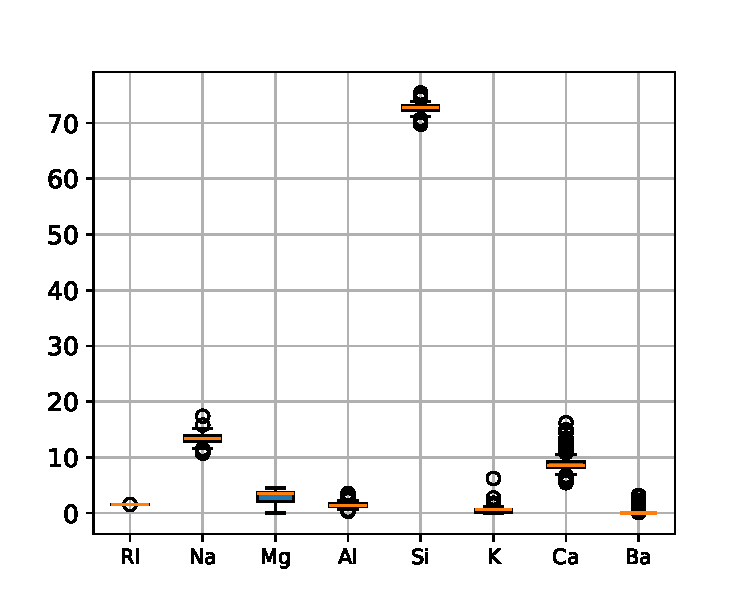
\includegraphics[width=\textwidth]{figures/boxplot_unstandardized}
			\caption{Unscaled boxplots of the refractive index (\texttt{RI}) and the 8 oxides.}
			\label{fig:unscaled-boxplots}
		\end{subfigure}
		\hspace*{0.02\textwidth}
		\begin{subfigure}{.49\textwidth}
			\centering
			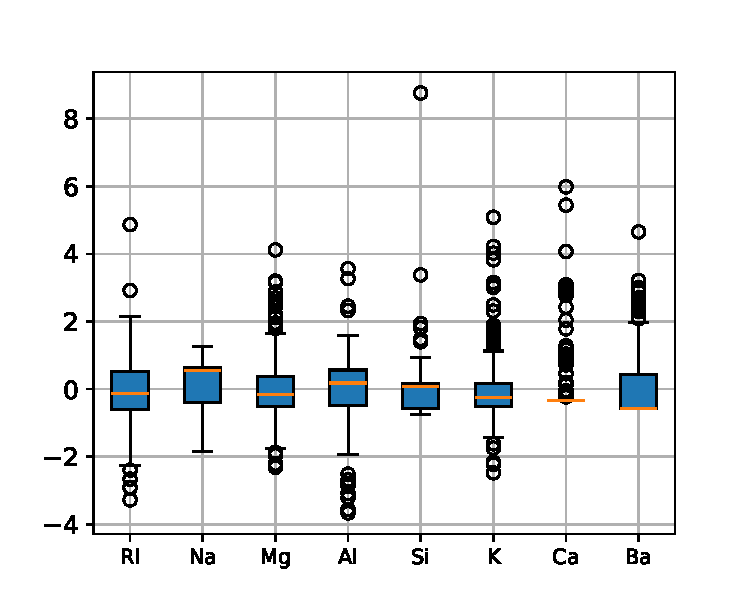
\includegraphics[width=\textwidth]{figures/boxplot_standardized}
			\caption{Scaled boxplots of the refractive index (\texttt{RI}) and the 8 oxides.}
			\label{fig:scaled-boxplots}
		\end{subfigure}
	\end{figure}

	\begin{figure}
		\centering
		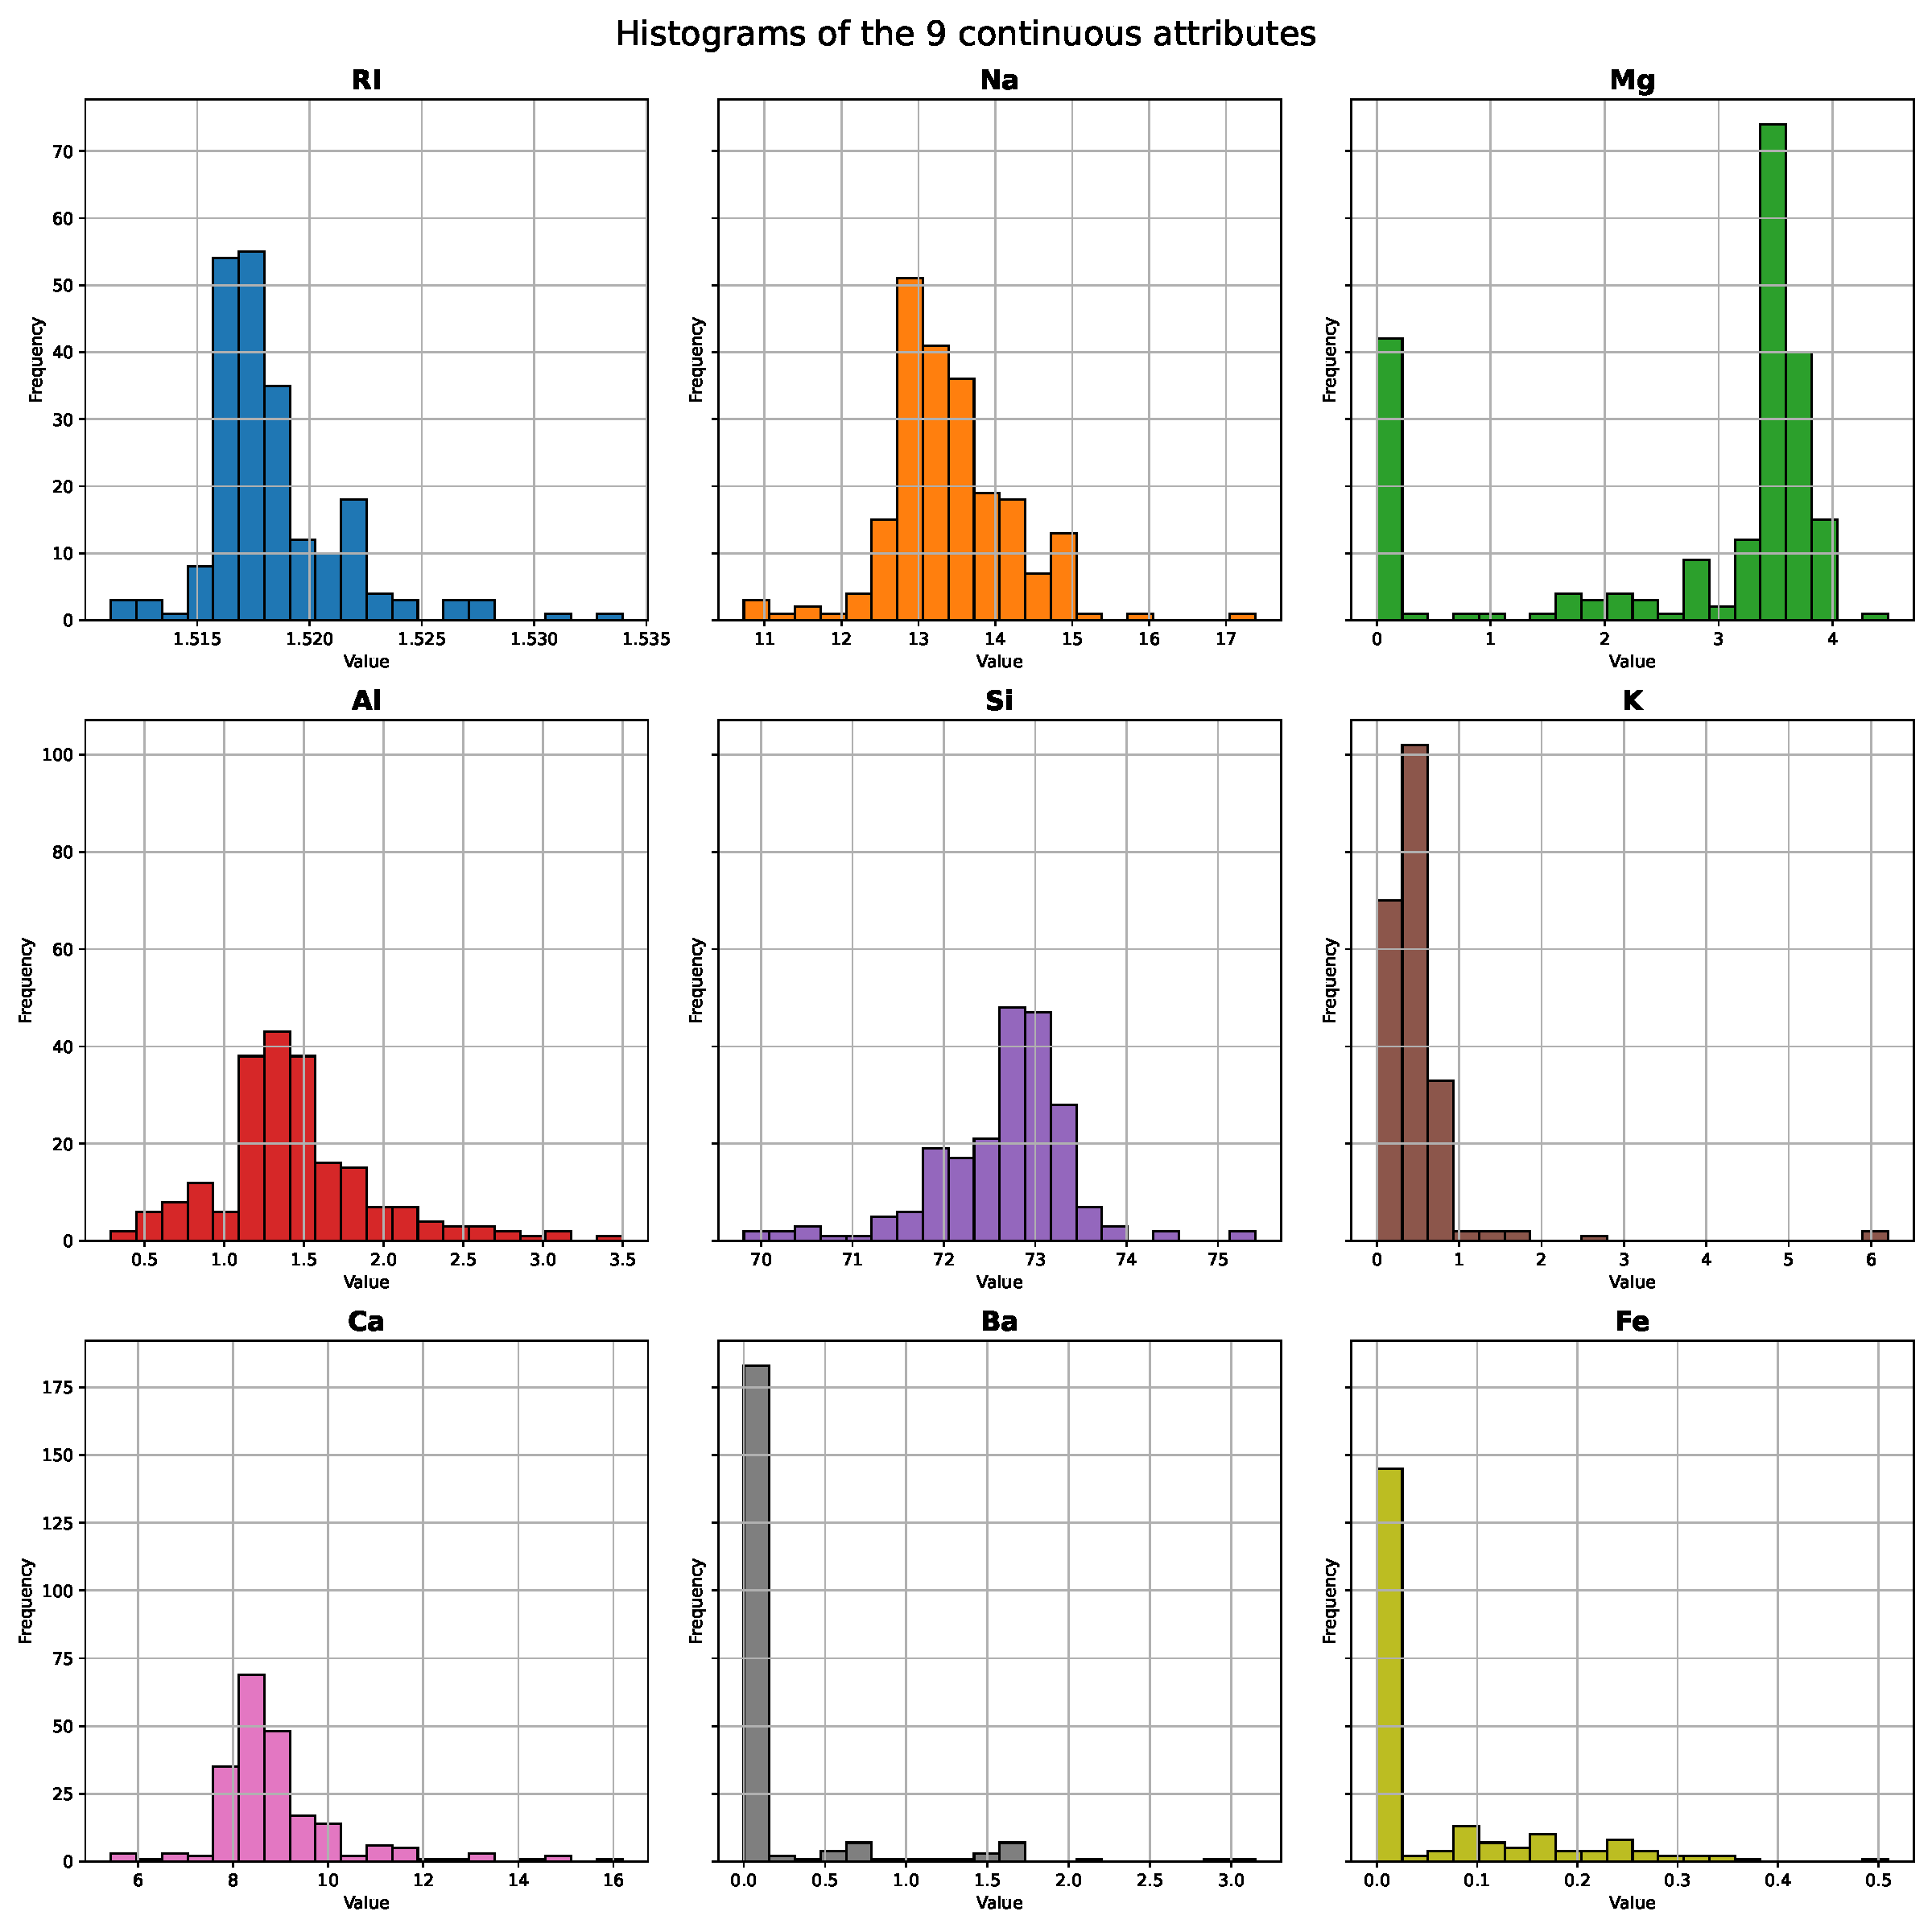
\includegraphics[width=.8\textwidth]{figures/histograms}
		\caption{Relative frequency histograms for the nine numerical attributes}
		\label{fig:histograms}
	\end{figure}

	\begin{table}
		\centering
		\begin{subtable}{0.65\textwidth}
			\begin{tabular}{r | *{6}{| r}}
				& \textbf{Mean} & \textbf{Std.} & \textbf{Min} & \textbf{Max} & \textbf{Skew} & \textbf{Kurtosis} \\ \hline\hline
				\texttt{RI} & 1.518 & 0.003 & 1.511 & 1.534 & 1.625 & 4.932 \\ \hline
				\texttt{Na} & 13.408 & 0.817 & 10.730 & 17.380 & 0.454 & 3.052 \\ \hline
				\texttt{Mg} & 2.685 & 1.442 & 0.000 & 4.490 & -1.153 & -0.410 \\ \hline
				\texttt{Al} & 1.445 & 0.499 & 0.290 & 3.500 & 0.907 & 2.061 \\ \hline
				\texttt{Si} & 72.651 & 0.775 & 69.810 & 75.410 & -0.730 & 2.968 \\ \hline
				\texttt{K} & 0.497 & 0.652 & 0.000 & 6.210 & 6.552 & 54.690 \\ \hline
				\texttt{Ca} & 8.957 & 1.423 & 5.430 & 16.190 & 2.047 & 6.682 \\ \hline
				\texttt{Ba} & 0.175 & 0.497 & 0.000 & 3.150 & 3.416 & 12.541 \\ \hline
				\texttt{Fe} & 0.057 & 0.097 & 0.000 & 0.510 & 1.754 & 2.662
			\end{tabular}
			\caption{Summary statistics.}
			\label{table:summary-stats}
		\end{subtable}
		\hspace*{0.02\textwidth}
		\begin{subtable}{.3\textwidth}
			\begin{tabular}{r|l|r|r}
				& \texttt{type}       & \textbf{Cnt.} & \textbf{Freq.} \\ \hline\hline
				1 & \texttt{BW-FP}      & 70 & 0.327 \\ \hline
				2 & \texttt{BW-NFP}     & 76 & 0.355 \\ \hline
				3 & \texttt{VW-FP}      & 17 & 0.079 \\ \hline
				4 & \texttt{VW-NFP}     & 0  & 0.000 \\ \hline
				5 & \texttt{containers} & 13 & 0.061 \\ \hline
				6 & \texttt{tableware}  & 9  & 0.042 \\ \hline
				7 & \texttt{headlamps}  & 29 & 0.136
			\end{tabular}
			\caption{Absolute and relative frequencies of \texttt{type}.}
			\label{table:frequencies}
		\end{subtable}
		\caption{Summary statistics of continuous variables and frequency distribution of glass \texttt{type}.}
	\end{table}


	\subsection{Correlation between attributes}

	\label{section:correlation}

	The correlation structure of the nine numerical attributes is summarised by the correlation-matrix
	heatmap (Figure~\ref{fig:correlation}).  Several clear patterns are visible in the \textit{linear} correlations:

	\begin{itemize}
	  \item \textbf{Strong positive correlation between refractive index and calcium:} As can be seen in Figure \ref{fig:individual-correlation}, RI and Ca have a large
	    positive linear association (Pearson $r \approx +0.81$). This indicates that samples with higher
	    calcium content tend to have larger refractive indices in this dataset.
	  \item \textbf{Notable negative correlation between RI and Si:} RI and Si are negatively correlated
	    ($r \approx -0.54$), so silica-rich samples tend to have somewhat lower RI values.
	  \item \textbf{Moderate correlations involving Mg, Al and Ba:} Mg is negatively correlated with both Ba
	    and Al (e.g. Mg--Ba $r\approx -0.49$, Mg--Al $r\approx -0.48$), while Al and Ba show a moderate
	    positive correlation (Al--Ba $r\approx +0.48$). Na and K show only weak-to-moderate associations
	    with other oxides (e.g. Na--Ba $r\approx +0.33$, Al--K $r\approx +0.33$).
	  \item \textbf{Generally weak correlations for Fe:} iron (Fe) has only small correlations with the other
	    variables (all $|r| \ll 0.5$).
	\end{itemize}

	These patterns have two important consequences for downstream analysis. First, several pairs/groups of
	variables show moderate-to-strong linear dependence (e.g. RI/Ca, Mg/Ba, Al/Mg). Such \textit{collinearity} can
	inflate variance of coefficient estimates in linear methods and makes interpretation of individual
	coefficients difficult. Second, the oxides are \textit{compositional} (the percentages sum to one), which
	can induce spurious correlations; standard multivariate techniques (PCA, regularised regression, or
	compositional transforms such as log-ratios) should be considered if the analysis requires interpretable
	linear relationships.

	For visualization and dimensionality reduction we used PCA (Section~\ref{section:pca}). The correlation structure above
	is consistent with the PCA loadings: PC1 places large positive weight on RI and Ca, and negative weight
	on Al and Si; PC2 emphasises Mg and Ba.  See Figure~\ref{fig:correlation} for the full matrix and the
	scatter example (RI vs Ca) that illustrates the strongest linear relationship identified above.

	\begin{figure}
		\centering
		\begin{subfigure}{.49\textwidth}
			\centering
			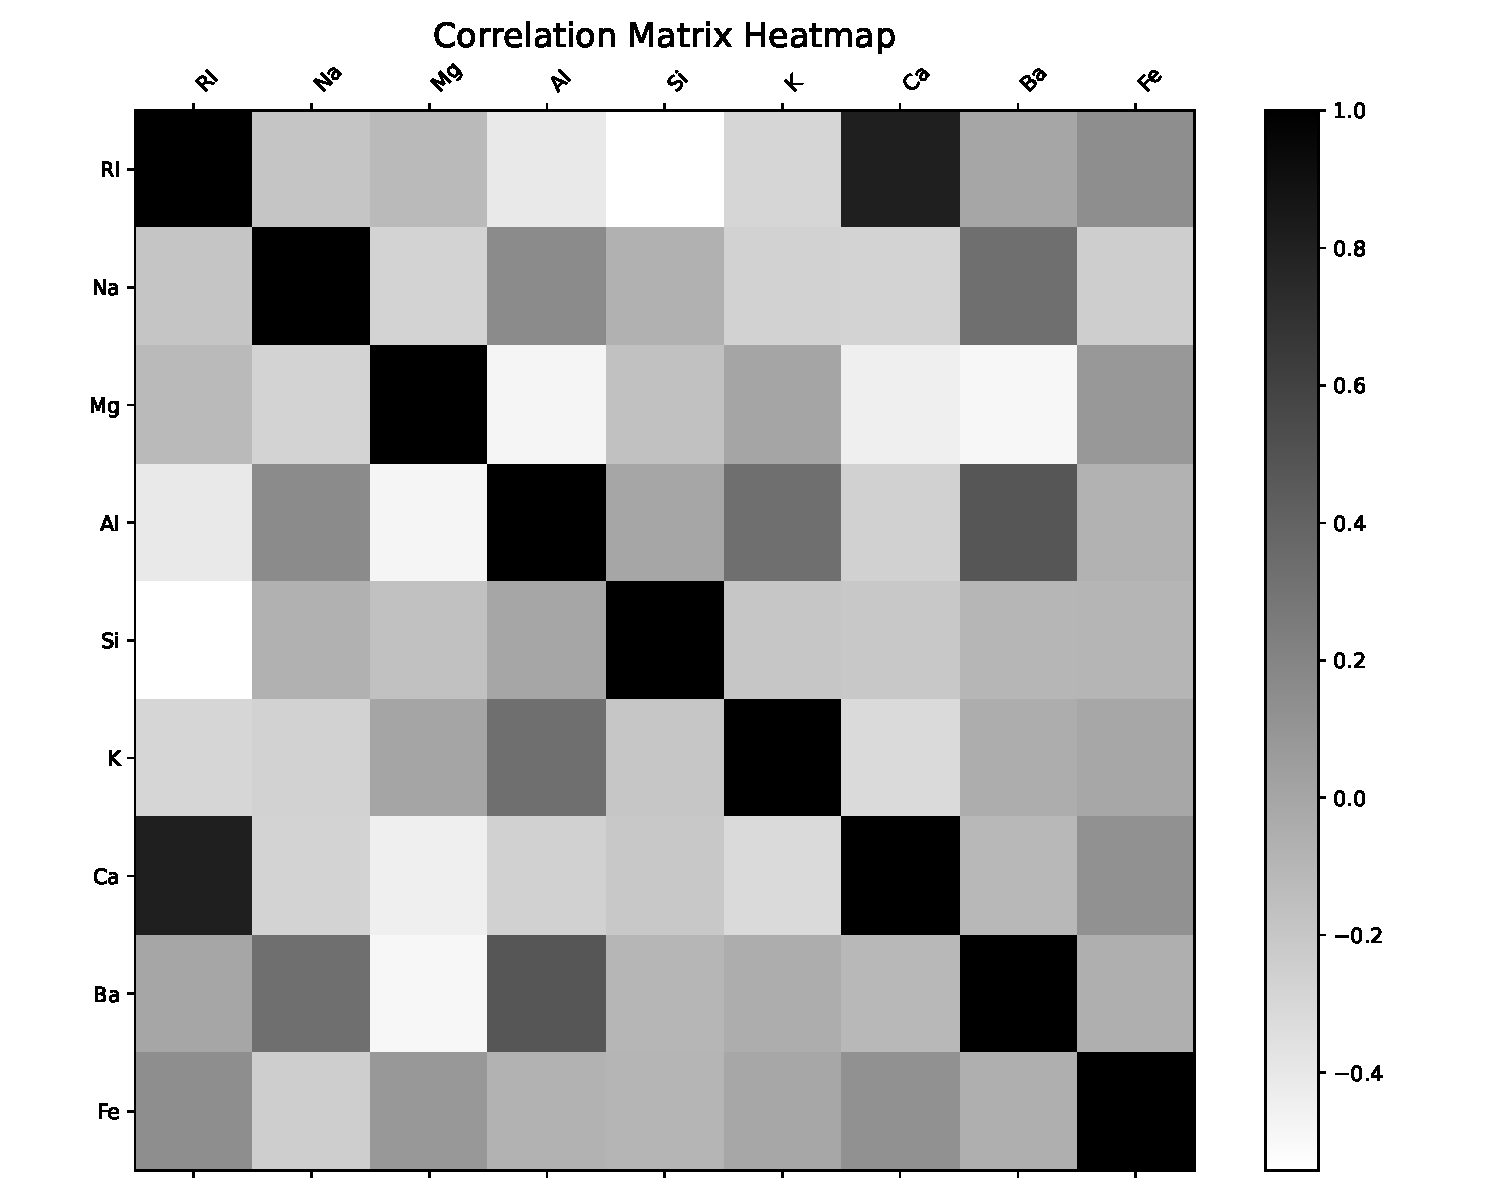
\includegraphics[width=\textwidth]{figures/correlation_matrix}
			\caption{Correlation matrix for the nine numerical attributes.}
			\label{fig:correlation}
		\end{subfigure}
		\begin{subfigure}{.49\textwidth}
			\centering
			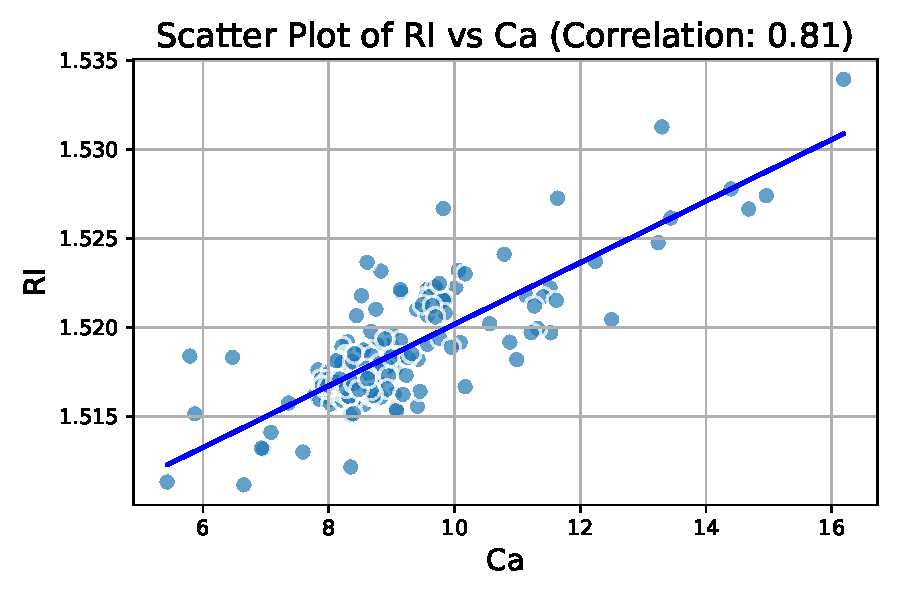
\includegraphics[width=\textwidth]{figures/scatter_RI_vs_Ca}
			\caption{Individual correlation between \texttt{RI} and \texttt{Ca}}
			\label{fig:individual-correlation}
		\end{subfigure}
		\caption{Whole correlation matrix and individual correlation between \texttt{RI} and \texttt{Ca}.}
	\end{figure}

	\section{Principal Component Analysis}

	\label{section:pca}

	\subsection{Need for standardisation}

	Since the attributes are expressed on different numerical scales (see Section \ref{section:scaling}), the variables are standardised by subtracting the mean and dividing by the standard deviation. This ensures that no single attribute dominates the analysis merely due to its scale.

	\subsection{Dimension reduction}

	\begin{figure}
		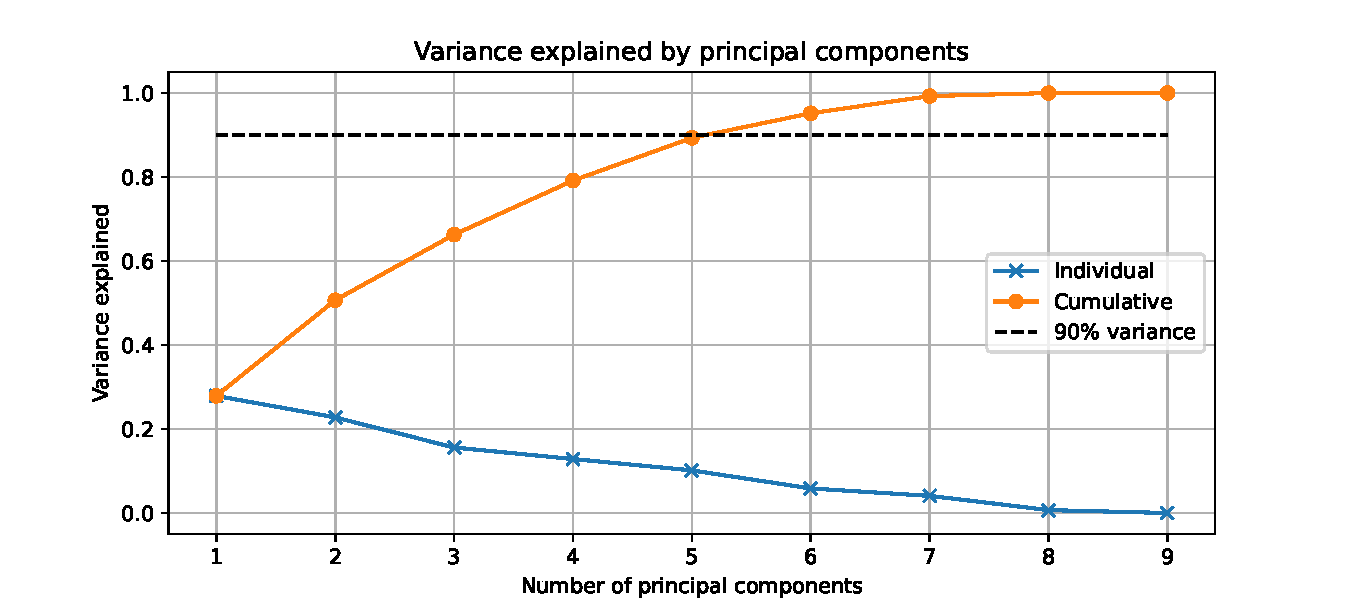
\includegraphics[width=.9\textwidth]{figures/pca_explained_variance}
		\caption{Explained (cumulative) variances for the 9 principal components $\bm{v}_0,\ldots,\bm{v}_8$}.
		\label{fig:explained-var}
	\end{figure}

	The goal is to reduce the original 9-dimensional dataset to an $M$-dimensional representation with $M < 9$, using the first $M$ principal components $\bm{v}_1,\ldots,\bm{v}_{M}$. As shown in Figure \ref{fig:explained-var}, selecting $M=5$ principal components explains \SI{89.31}{\percent} of the total variance. By increasing the dimensionality to $M=7$, as much as \SI{99.27}{\percent} of the variance can be retained, essentially preserving almost all of the original information.

	While $M=7$ captures nearly all of the variance, the marginal gain in explained variance beyond the first five components is relatively small compared to the added complexity. Retaining five dimensions reduces computational cost, simplifies subsequent analysis, and removes noise while still preserving the majority of the data's variability. We conclude that choosing $M=5$ provides a balance between dimensionality reduction and information retention.

	\subsection{Principal directions}

	The \textit{principal directions} of the first $M$ principal components are defined by the eigenvectors $\bm{v}_i$ that span the subspace of reduced dimensionality. These vectors form the transformation matrix $\bm{V}_M$, which is applied to the standardised data $\tilde{\bm{X}}$ to obtain the projected representation $\bm{B} = \bm{V}_M \tilde{\bm{X}}$. The new coordinates $\bm{B}$ capture the structure of the data in fewer dimensions while emphasising the directions of greatest variance. Based on the loadings in Table \ref{table:loadings} and the corresponding visualisation in Figure \ref{fig:pc-components}, we interpret the first 5 principal components:

	\begin{table}
		\centering
		\begin{tabular}{r | *{5}{|r}}
			\textbf{Variable} & $\textbf{PC}_1$ & $\textbf{PC}_2$ & $\textbf{PC}_3$ & $\textbf{PC}_4$ & $\textbf{PC}_5$ \\ \hline\hline
			\texttt{RI} & \num{0.545}     &          -0.286 &           0.087 &          -0.147 &          -0.074 \\
			\texttt{Na} & -0.258          &          -0.270 &          -0.385 &          -0.491 &           0.154 \\
			\texttt{Mg} & 0.111           &           0.594 &           0.008 &          -0.379 &           0.124 \\
			\texttt{Al} & -0.429          &          -0.295 &           0.329 &           0.138 &           0.014 \\
			\texttt{Si} & -0.229          &           0.155 &          -0.459 &           0.653 &           0.009 \\
			\texttt{K} & -0.219          &           0.154 &           0.663 &           0.039 &          -0.307 \\
			\texttt{Ca} & 0.492           &          -0.345 &          -0.001 &           0.276 &          -0.188 \\
			\texttt{Ba} & -0.250          &          -0.485 &           0.074 &          -0.133 &           0.251 \\
			\texttt{Fe} & 0.186           &           0.062 &           0.284 &           0.230 &           0.873
		\end{tabular}
		\caption{The principal directions (a.k.a. the \textit{loadings}) of the first $M=5$ principal components $\text{PC}_i = \bm{v}_i$ in the rotation matrix $\bm{V}_M$. Larger absolute values indicate stronger influence of a variable on a given component.}
		\label{table:loadings}
	\end{table}

	\begin{figure}
		\centering
		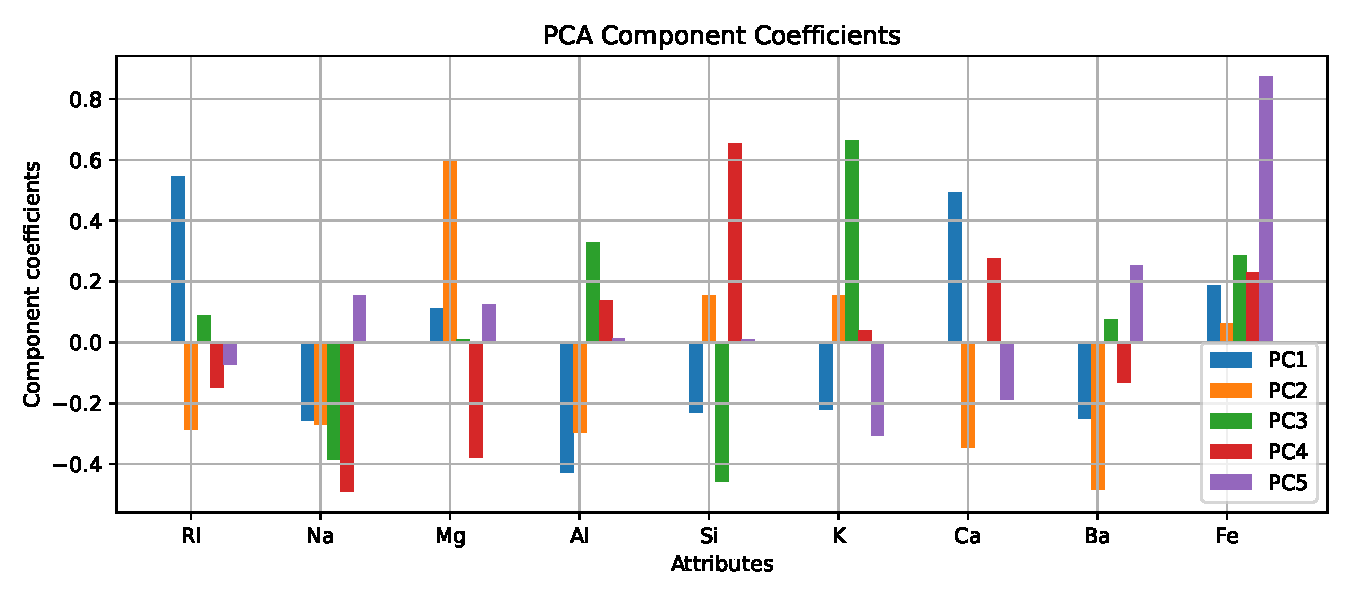
\includegraphics[width=.99\textwidth]{figures/pca_component_coefficients}
		\caption{Loadings of the original variables on the first five principal components. Positive and negativ values indicate the \textit{direction} of influence, while the magnitude reflects the \textit{strength} of the contribution.}
		\label{fig:pc-components}
	\end{figure}

	\begin{itemize}
		\item The first principal component ($\text{PC}_1$) is most strongly influenced by \texttt{RI} and \texttt{Ca}, which carry positive loadings, and negatively by \texttt{Al} and \texttt{Si}. This suggests that $\text{PC}_1$ captures a trade-off between refractive index and calcium content versus aluminium and silicon.

		\item The second principal component ($\text{PC}_2$) assigns a large positive loading to \texttt{Mg}, while strongly down-weighting \texttt{Ba} and, to a lesser degree, \texttt{Na}. This indicates that $\text{PC}_2$ primarily reflects a contrast between magnesium concentration and the presence of barium and sodium.

		\item The third principal component ($\text{PC}_3$) is dominated by a large positive loading for \texttt{K}, balanced by strong negative contributions from \texttt{Si} and \texttt{Na}. This points to a dimension that separates potassium-rich compositions from those with higher silica and sodium content.

		\item The fourth principal component ($\text{PC}_4$) shows high positive contributions from \texttt{Si}, \texttt{Ca}, and \texttt{Fe}, with negative influence from \texttt{Mg} and \texttt{Na}. It therefore captures variation where higher levels of silicon, calcium, and iron occur together in opposition to magnesium and sodium.

		\item Finally, the fifth principal component ($\text{PC}_5$) is characterised by a dominant positive loading for \texttt{Fe}, while moderately influenced by \texttt{Ba} and negatively by \texttt{K}. This indicates that $\text{PC}_5$ primarily isolates variation in iron concentration, with some contribution from the balance between barium and potassium.
	\end{itemize}

	\subsection{Projected data}

	\subsubsection{Biplots}

	The projection of the standardized dataset onto the principal component axes produces a lower-dimensional representation that can be visualized in two-dimensional \textit{biplots}. In these plots:

	\begin{itemize}
		\item Each point corresponds to a \textit{score}, representing the coordinates of an original observation in the space spanned by the selected principal components. The scores have been \textit{rescaled} to the interval $[-1,1]$ to facilitate comparison with the arrows, representing variable loadings.
		\item The arrows correspond to the \textit{loadings}, i.e., the contributions of the original variables to the principal components. The direction of an arrow indicates how the variable influences the component axes, and its length reflects the magnitude of this influence.
	\end{itemize}

	Together, scores and loadings allow for simultaneous interpretation of both the observations and the variables.

	\subsubsection{Interpretation}

	Figure~\ref{fig:biplots} shows two biplot visualizations. In the first biplot (PC1 vs.\ PC2), which captures \SI{50}{\percent} of the variance, the dominant trends in the data are visible, and some separation between glass types can be observed. We can, for example, see a clear separation of headlamps, who on average score low on PC1 and have about a zero-loading for PC2. The building and vehicle windows, on the other hand, show significant overlap and can thus not be distinguished from each other by just looking at the first two principal components.

	The loadings indicate that the separation of classes along the axes is largely driven by specific chemical compositions; for example, PC1 contrasts samples with high \texttt{RI} and \texttt{Ca} against those with higher \texttt{Al} and \texttt{Si}, explaining why some classes separate along this component.

	\begin{figure}
		\centering
		\begin{subfigure}{0.49\textwidth}
			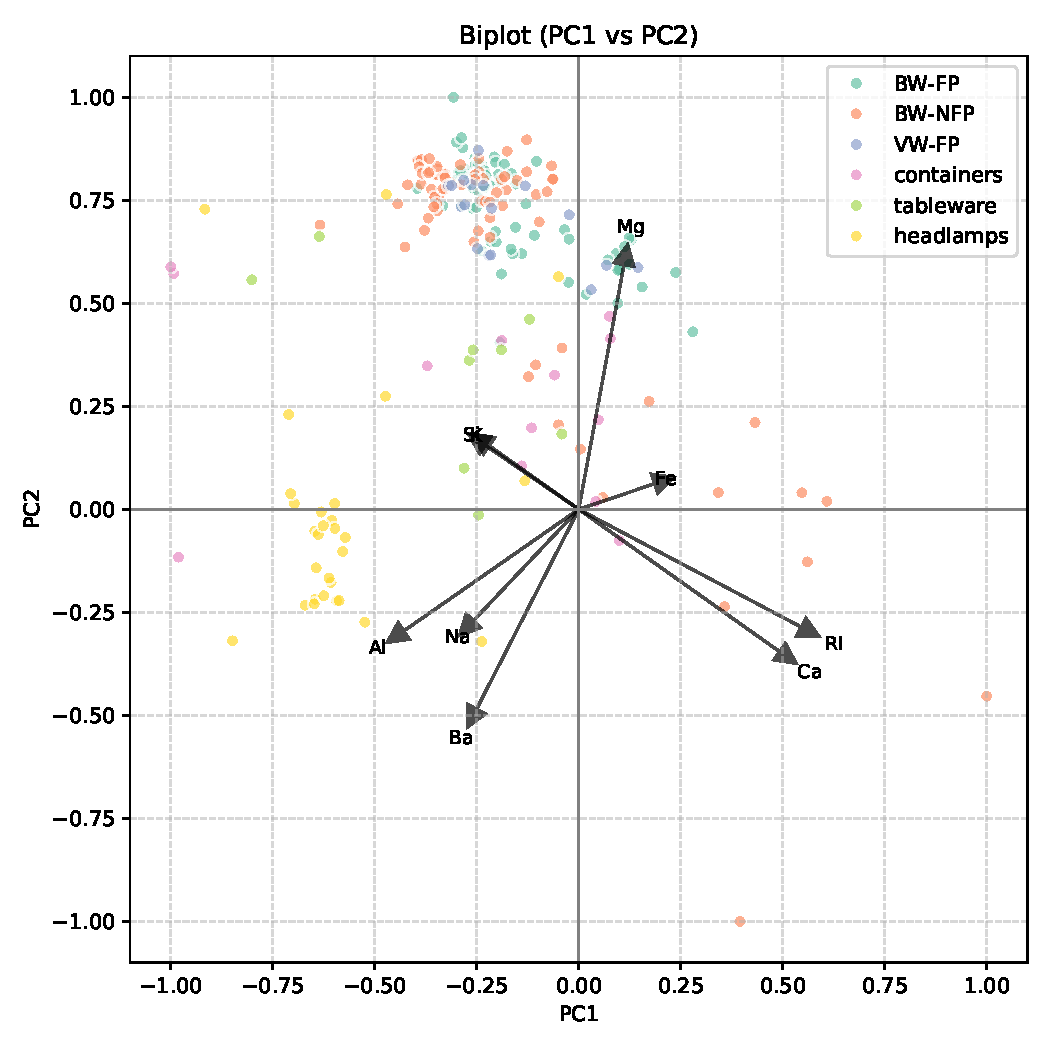
\includegraphics[width=\linewidth]{figures/pca_biplot_pc1_pc2.pdf}
			\caption{PC1 vs PC2}
			\label{fig:biplot_pc1_pc2}
		\end{subfigure}
		\hfill
		\begin{subfigure}{0.49\textwidth}
			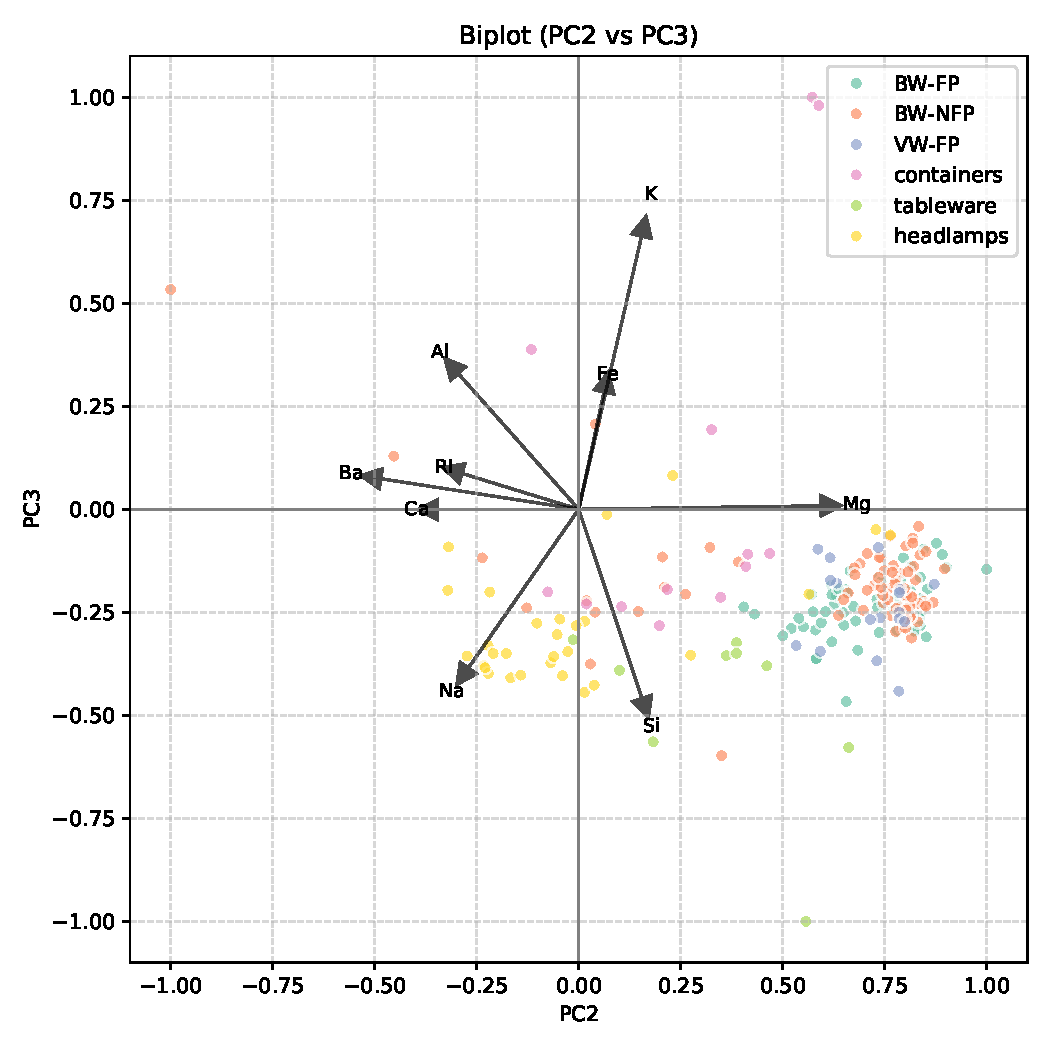
\includegraphics[width=\linewidth]{figures/pca_biplot_pc2_pc3.pdf}
			\caption{PC2 vs PC3}
			\label{fig:biplot_pc1_pc3}
		\end{subfigure}
		\caption{Biplots of the glass dataset showing both projected samples (colored by class) and variable loadings.}
		\label{fig:biplots}
	\end{figure}

	\section{Discussion}
	\paragraph{Summary of main findings.}
	From the descriptive analysis and visualisations we draw the following principal conclusions. The dataset
	contains $N=214$ samples described by nine numerical attributes (\texttt{RI} + eight oxides). There are no
	missing values. Many variables are skewed (notably \texttt{K} and \texttt{Ba}) and some have occasional extremes
	(especially \texttt{Ba} and \texttt{Ca}); \texttt{Mg} shows a bimodal-like pattern across the dataset. The class distribution is
	imbalanced: building-window classes dominate (70 and 76 samples), headlamps are moderately represented
	(29), while container/tableware classes are small (13 and 9 samples) and one of the UCI classes is
	absent in our download. The correlation analysis (Section~\ref{section:correlation}) reveals substantial
	linear dependence (e.g. \texttt{RI}--\texttt{Ca} $r\approx +0.81$, \texttt{RI}--\texttt{Si} $r\approx -0.54$, \texttt{Mg}--\texttt{Ba} $r\approx -0.49$),
	which motivated the PCA and dimensionality-reduction work in Section~\ref{section:scaling}.

	\paragraph{Feasibility of the classification aim.}
	Our baseline supervised experiments (Random Forest and logistic regression on standardised oxide-only
	features) show that the multi-class classification task is feasible but non-trivial. The Random Forest
	achieved a test accuracy of approximately 0.674 on the held-out set and a 5-fold cross-validated
	mean accuracy of around \SI{0.748(0.029)}{}. The PCA biplots
	indicate that some classes (notably the two building-window classes) substantially overlap in the
	leading principal-component space and are therefore inherently harder to separate; by contrast, the
	headlamps class appears relatively well separated along PC1/PC2. Small sample sizes for containers and
	tableware make reliable classification for those classes challenging without further data or targeted
	rebalancing.

	\paragraph{Actionable next steps and points of attention.}
	Based on the visual and numerical diagnostics we consider the following steps:

	\begin{enumerate}
	  \item \textbf{Address skewness and extremes:} apply robust transformations (e.g. log or Box--Cox for
	    strictly positive oxides), and consider robust estimators or tree-based models
	    that handle outliers naturally.
	  \item \textbf{Reduce redundancy:} use PCA (or regularised models) to control multicollinearity in linear
	    approaches; alternatively, select a compact subset of chemically interpretable predictors.
	  \item \textbf{Compositional caution:} because oxide measurements are parts of a composition,
	  compositional data methods (e.g. log-ratio transforms) could be considered.
	  \item \textbf{Class imbalance:} the class imbalance should be handled with care.
	\end{enumerate}

	Taken together, these steps should increase both predictive performance and interpretability. The
	baseline results and the PCA visualisations indicate that the classification objective is realistic, but
	substantial care is needed for small classes and for correct preprocessing of compositional and skewed
	measurements.

	\paragraph{Limitations.} The main limitations at this stage are (i) class imbalance and small sample
	counts for some classes, (ii) compositional structure that can bias naive correlation-based interpretations,
	and (iii) sensitivity to outliers for some attributes (Ba, Ca, K). These caveats should guide model
	selection and evaluation in the next project phase.



	\section*{Use of GenAI}
	For the sake of transparency, the project used generative-AI tools in a limited and documented manner:
	GenAI assisted primarily with \emph{work-organisation suggestions} and language polishing when going from draft to final report. All quantitative analyses, figures, and
	numerical results reported in this document were produced by the code in the repository and the
	authors' own computations were \emph{not} fabricated by GenAI. It should be noted that some team members make use of the VSCode Copilot code completion to speed up their programming work. Where GenAI suggestions
	were used, the group reviewed and validated them against the code outputs and figures before inclusion.

	\bibliography{citations}
	\bibliographystyle{unsrt}

	\vspace*{1cm}
	\appendix

	\LARGE\bfseries Appendix

	\normalsize\normalfont

	\section{Repository and supplementary materials}
	The full notebook, scripts, and generated figures for this project are available in the project repository:
	\begin{quote}
	\url{https://github.com/schependom/DTU_machine-learning-projects/tree/main}
	\end{quote}
	This repository contains the data-loading and analysis code that produced the tables and figures cited
	above (see the \texttt{figures/} folder for the PDF outputs referenced in the report).
%
%

%	\section{Test}

\end{document}
